% !TEX engine = xelatex

\documentclass[12pt,aps,pra,notitlepage]{revtex4-1}
\usepackage{amsmath,amssymb}
\usepackage{xeCJK}
\usepackage{graphicx}
\setCJKmainfont{STSong}
\DeclareMathOperator{\tr}{tr}
\begin{document}

\title{大作业}
\maketitle
\begin{center}
  12月10号截止。从以下两题中选做一题。
\end{center}
\begin{enumerate}
  \item 三角晶格反铁磁序的相变。

  考虑一个三维三角晶格:在$xy$平面内格点形成三角晶格,在$z$方向形成该三角晶格的周期性排列。我们用$iz$标记每个格点,其中$i$标记三角晶格的格点,$z$标记$z$坐标。在每个格点上放置一个伊辛自旋$\sigma_{iz}$,自旋之间的相互作用如下:
  \[H=J\sum_{\langle ij\rangle z}\sigma_{iz}\sigma_{jz}-J\sum_{iz}\sigma_{iz}\sigma_{i,z+1}.\]
  即在三角晶格面内为最近邻的反铁磁相互作用;在面间为铁磁相互作用。

  这样一个模型在低温下会形成一个反铁磁长程序:在三角晶格面内形成如图~\ref{fig:order}所示的长程序,在面间形成铁磁长程序。这个长程序的序参量可以采用如下定义:我们用$m_1$, $m_2$, $m_3$分别表示三角晶格上三套子格上的平均磁化(三套子格指图中的a,b,c三类不等价的格点,每个三角形的三个顶点都各属于一个子格);定义一个复的序参量$\psi=me^{i\theta}$:
  \[\psi=m_1+m_2e^{i4\pi/3}+m_3e^{-i4\pi/3}.\]

  \begin{enumerate}
    \item 写出$\psi=me^{i\theta}$在晶格平移、旋转对称性及自旋对称性$\sigma\rightarrow-\sigma$下的变换形式。
    \item 证明对称性允许的Landau-Ginzberg理论的形式,展开到有$\theta$依赖关系的最低阶的形式如下:
    \[F=(\nabla m)^2+rm^2+um^4+vm^6+v'm^6\cos(6\theta).\]
    \item 计算$v'$在$\epsilon=4-D$展开下的标度维数(展开到$\epsilon$的第一阶),并以此判断$v'$是relevant还是irrelevant perturbation。
    \item 根据这个展开结果,这个相变的普适类是什么?

    提示:本题源自S. V. Isakov and R. Moessner, Phys. Rev. B {\bf 68}, 104409 (2003).
  \end{enumerate}

  \begin{figure}
    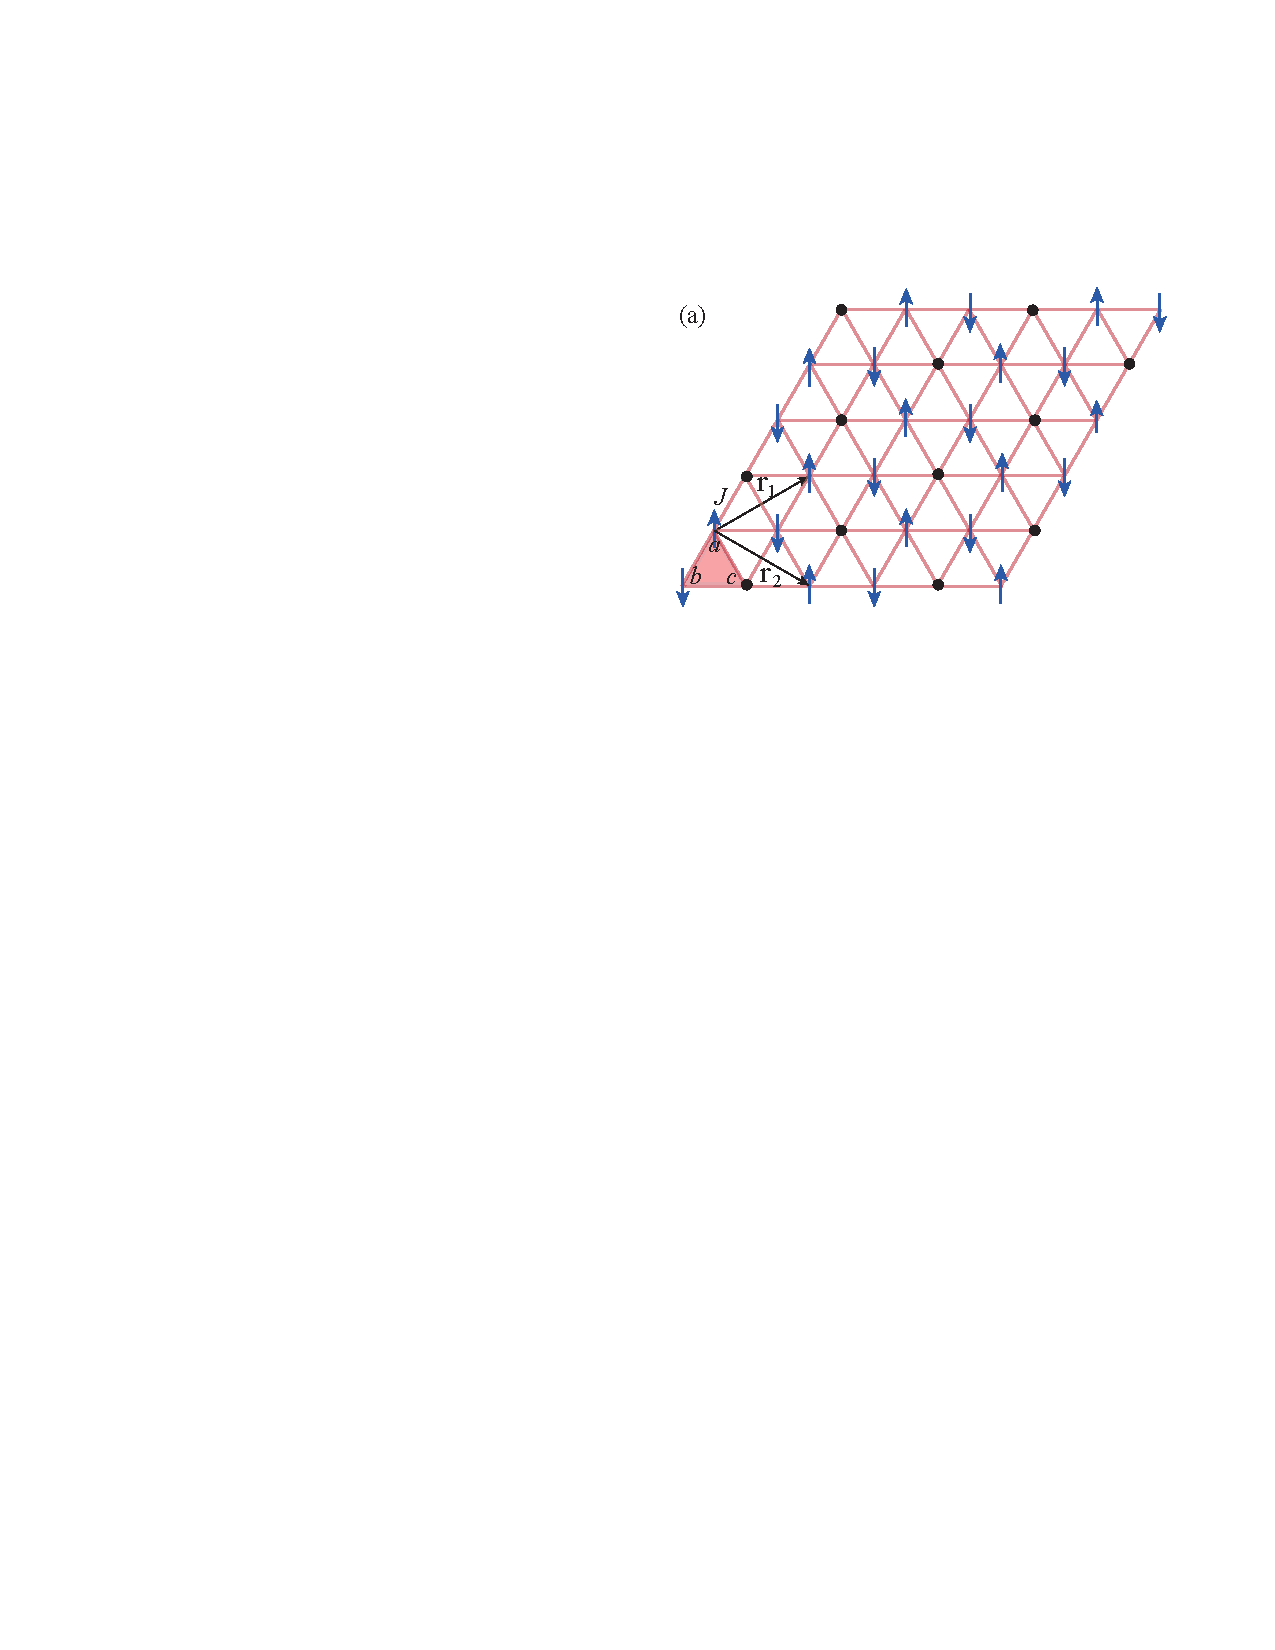
\includegraphics{triafm}
    \caption{三角晶格上的反铁磁伊辛长程序}
    \label{fig:order}
  \end{figure}

  \item 二维伊辛模型的数值模拟。

  利用Wolff算法编写一个二维正方格点上伊辛模型的数值模拟程序。
  \begin{enumerate}
    \item 计算Binder cumulant并以此确定相变点的位置。
    \item 测量不同系统大小及温度下的磁化,代入标度函数,验证利用二维伊辛模型的标度指数(见教材第13.4节)可以令数据落到一条普适曲线上。

    提示:利用课上讲的临界点附近的标度律,用临界标度指数构造出两个在标度变换下无量纲的组合$ML^a$和$tL^b$,这里$a$和$b$由二维伊辛模型的标度指数确定。在不同的温度和系统大小下测量磁化,并验证这两个无量纲量之间满足一个普适的函数关系:
    \[ML^a = f(tL^b).\]
    这里二维伊辛模型的标度指数认为是已知的。
  \end{enumerate}
\end{enumerate}
\end{document}
